\section{A Symbolic Heap}
\label{sec:symheap}
A \emph{symbolic heap}, as defined in this work, is a tuple
$(\cfgnt{L}\ \cfgnt{R}\ \phi\ \eta)$, indicating a \emph{location map}
$\cfgnt{L}$, a \emph{reference map} $\cfgnt{R}$, a \emph{path condition} $\phi$, and an \emph{environment} $\eta$.  Given a reference $r$ in the heap,
$\cfgnt{L}(r) = \{(\phi\ \cfgnt{l})\ ...\}$ is the guarded value set
associated with $r$. The constraint associated with each
location is a guard representing the conditions under which the
associated reference maps to the given location. By definition, any
location appears at most once in any given value set. Unions of value
sets containing the same location are resolved by forming a
disjunction of the constraints from each set. $\cfgnt{R}(\cfgnt{l},
\cfgnt{f}) = \cfgnt{r}$ is the reference associated with the given
location-field pair in the heap.

\begin{figure}[t]
\begin{center}
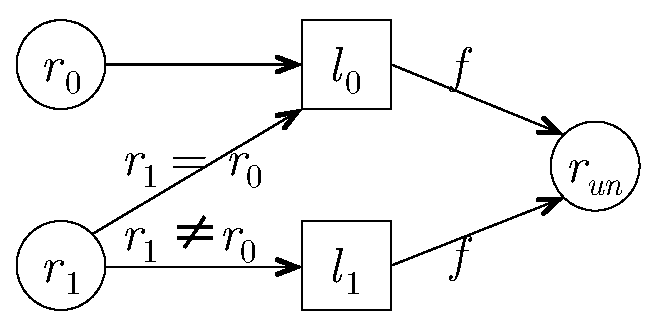
\includegraphics[scale=0.5]{../figs/simple_heap_scratch.pdf}
\end{center}
\caption{Example Symbolic Heap}
\label{fig:exampleHeap}
\end{figure}

The path condition is a predicate of the program variables. The environment is a partial function so $\eta(\cfgnt{x}) = \cfgnt{r}$ is the reference
$\cfgnt{r}$ associated with variable $\cfgnt{x}$. The notation
$\eta^\prime = \eta[\cfgnt{x} \mapsto \cfgnt{v}]$ defines a new
partial function $\eta^\prime$ that is the same as $\eta$ except that
the variable $\cfgnt{x}$ now maps to $\cfgnt{v}$. This notation for update is used with $\cfgnt{L}$ and $\cfgnt{R}$ as well. 

Conceptually, the symbolic heap may be thought of as a bipartite
graph. \figref{fig:exampleHeap} shows an example symbolic heap
graph. References are represented by circles and locations are
represented by squares. Arrows leaving references correspond to the
guarded value sets returned by the $\cfgnt{L}$ function, and arrows
leaving the squares correspond to the $\cfgnt{R}$ function. The
reference $\cfgnt{r}_1$ in the figure has two members in its guarded value set,
so the location pointed to by $\cfgnt{r}_1$ depends on its aliasing
relationship to $\cfgnt{r}_0$.

The reference $\cfgnt{r}_\mathit{un}$ is a special reference to
indicate something that has yet to be initialized. In general, every
symbolic heap contains two special locations, null
($\cfgnt{l}_\mathit{null}$), and uninitialized
($\cfgnt{l}_\mathit{un}$), with corresponding references
$\cfgnt{r}_\mathit{null}$ and $\cfgnt{r}_\mathit{un}$ where
$\cfgnt{L}(\cfgnt{r}_\mathit{null}) =
\{(\cfgt{true}\ \cfgnt{l}_\mathit{null})\}$ and
$\cfgnt{L}(\cfgnt{r}_\mathit{un}) =
\{(\cfgt{true}\ \cfgnt{l}_\mathit{un})\}$.

A \emph{well-formed} symbolic heap is \emph{deterministic} and \emph{type consistent}. Determinism means a reference in $(\cfgnt{L}\ \cfgnt{R}\ \phi\ \eta)$ cannot point to multiple locations simultaneously: 
$
\forall \cfgnt{r} \in \cfgnt{L}^\leftarrow\ (\forall (\phi\ \cfgnt{l}),(\phi^\prime\ \cfgnt{l}^\prime) \in \cfgnt{L}(r)\ (
(\cfgnt{l} \neq \cfgnt{l}^\prime \vee \phi \neq \phi^\prime) \Rightarrow (\phi \wedge \phi^\prime = \cfgt{false}))
$
where $\cfgnt{L}^\leftarrow$ is the pre-image of $\cfgnt{L}$.
Type consistent means that all locations in a guarded value set from a reference have the same type\footnote{Although not treated in this presentation, the concept naturally extends to polymorphic languages}:
$\forall \cfgnt{r} \in \cfgnt{L}^\leftarrow\ (\forall (\phi\ \cfgnt{l}),(\phi^\prime\ \cfgnt{l}^\prime) \in \cfgnt{L}(r)\ (
(\mathrm{Type}\lp\cfgnt{l}\rp = \mathrm{Type}\lp\cfgnt{l}^\prime\rp)))$

\section{Operational Semantics}
This paper defines symbolic initialization using
a small-step operational semantics in the context of a syntactic machine with a CESK architecture~\cite{Felleisen:1992, saints-MS}. The
surface  syntax  (input) and machine  syntax (state) are shown
in~\figref{fig:syntax}. The machine syntax omits the list based syntactic structures for the partial functions in the heap etc.  Terminals are in bold face while non-terminals
are italicized. Ellipses indicate zero or more repetitions. Tuples
omit the commas for compactness.

\begin{figure}
\begin{center}
\cfgstart
\cfgrule{P}{\lp $\mu$ \lp \cfgnt{C} \cfgnt{m}\rp\rp}
\cfgrule{$\mu$}{(\cfgnt{CL} ...)}
\cfgrule{T}{\cfgt{bool} \cfgor \cfgnt{C}}
\cfgrule{CL}{\lp\cfgt{class} \cfgnt{C} \lp\lb\cfgnt{T} \cfgnt{f}\rb ...\rp \lp\cfgnt{M} ...\rp}
\cfgrule{M}{\lp\cfgnt{T} \cfgnt{m} \lb\cfgnt{T} \cfgnt{x}\rb\  e\rp}
\cfgrule{e}{\cfgnt{x}
\cfgor{\lp\cfgt{new} \cfgnt{C}\rp}
\cfgor{\lp\cfgnt{e} \cfgt{\$} \cfgnt{f}\rp}
\cfgor{\lp\cfgnt{x} \cfgt{\$} \cfgnt{f} \cfgt{:=} \cfgnt{e}\rp}
\cfgor{\lp\cfgnt{e} \cfgt{=} \cfgnt{e}\rp}}
\cfgorline{\lp\cfgt{if} \cfgnt{e} \cfgnt{e} \cfgt{else} \cfgnt{e}\rp 
\cfgor {\lp\cfgt{var} \cfgnt{T} \cfgnt{x} \cfgt{:=} \cfgnt{e} \cfgt{in} \cfgnt{e}\rp}
\cfgor {\lp\cfgnt{e} \cfgt{@} \cfgnt{m} \cfgnt{e} \rp}}
\cfgorline{\lp\cfgnt{x} \cfgt{:=} \cfgnt{e}\rp
\cfgor{\lp\cfgt{begin} \cfgnt{e} ...\rp}
\cfgor{\cfgnt{v}}}
\cfgrule{x}{\cfgt{this} \cfgor \cfgnt{id}}
\cfgrule{f,m,C}{\cfgnt{id}}
%\cfgrule{m}{\cfgnt{id}}
%\cfgrule{C}{\cfgnt{id}}
\cfgrule{v}{\cfgnt{r} \cfgor \cfgt{null} \cfgor \cfgt{true} \cfgor \cfgt{false} \cfgor \cfgt{error}}
\cfgrule{r}{\cfgt{number}}
\cfgrule{id}{\cfgt{variable-not-otherwise-mentioned}}
\cfgend
\end{center}
\caption{The Javalite surface syntax.}
\label{fig:surface-syntax}
\end{figure}

\begin{figure}
\begin{center}
\cfgstart
\cfgrule{e}{\lp ... \cfgor \lp \cfgnt{v} \cfgt{@} \cfgnt{m} \cfgnt{v} \rp\rp}
%\cfgrule{object}{ (\cfgnt{C} [ \cfgnt{f} \cfgnt{loc} ] ...) }
%\cfgrule{hv}{ (\cfgnt{v} \cfgnt{object})}
\cfgrule{$\phi$}{\cfgnt{constraint}}
\cfgrule{l}{\cfgt{number}}
%\cfgrule{h}{(\cfgnt{mt}\ (\cfgnt{h}\ [\cfgnt{loc} $\rightarrow$ \cfgnt{hv}]) )}
\cfgrule{$\eta$}{(\cfgnt{mt}\ ($\eta$ [\cfgnt{x} $\rightarrow$ \cfgnt{loc}]))}
\cfgrule{s}{\lp$\mu$ \cfgnt{L} \cfgnt{R} \cfgnt{g} $\eta$ \cfgnt{e} \cfgnt{k}\rp}
\cfgrule{k}{\cfgt{end}}
\cfgorline{\lp \cfgt{*} \cfgt{\$} \cfgnt{f} $\rightarrow$ \cfgnt{k}\rp}
\cfgorline{\lp \cfgt{*} \cfgt{@} \cfgnt{m} \lp \cfgnt{e} ... \rp $\rightarrow$ \cfgnt{k} \rp}
\cfgorline{\lp \cfgnt{v} \cfgt{@} \cfgnt{m} \cfgnt{v} \cfgt{*} \lp \cfgnt{e} ... \rp $\rightarrow$ \cfgnt{k} \rp}
\cfgorline{\lp \cfgt{*} \cfgt{=} \cfgnt{e} $\rightarrow$ \cfgnt{k}\rp}
\cfgorline{\lp \cfgt{v} \cfgt{=} \cfgnt{*} $\rightarrow$ \cfgnt{k}\rp}
\cfgorline{\lp \cfgt{x} \cfgt{:=} \cfgnt{*} $\rightarrow$ \cfgnt{k}\rp}
\cfgorline{\lp \cfgt{x} \cfgt{\$} \cfgnt{f}  \cfgt{:=} \cfgnt{*} $\rightarrow$ \cfgnt{k}\rp}
\cfgorline{\lp \cfgt{if} \cfgnt{*} \cfgnt{e} \cfgt{else} \cfgnt{e} $\rightarrow$ \cfgnt{k} \rp}
\cfgorline{\lp\cfgt{var} \cfgnt{T} \cfgnt{x} \cfgt{:=} \cfgnt{*} \cfgt{in} \cfgnt{e}  $\rightarrow$ \cfgnt{k} \rp}
\cfgorline{\lp\cfgt{begin}  \cfgnt{*} \lp \cfgnt{e} ...\rp $\rightarrow$ \cfgnt{k} \rp}
\cfgorline{\lp\cfgt{pop} $\eta$ \cfgnt{k}\rp}
\cfgend
\end{center}
\caption{The machine syntax for Javalite.}
\label{fig:machine-syntax}
\end{figure}

\begin{figure}[t]
\begin{center}
\begin{tabular}{c}
\scalebox{0.9}{\usebox{\boxSurface}} \\
(a) \\\\
\scalebox{0.9}{\usebox{\boxMachine}} \\
(b)
\end{tabular}
\end{center}
\caption{ (a) The surface syntax. (b) The machine syntax.}
\label{fig:syntax}
\end{figure}

A program, $\cfgnt{P}$, is a registry of classes, $\mu$, with
a tuple indicating a class, $\cfgnt{C}$, and a method, $\cfgnt{m}$,
where execution starts. For simplicity in presentation, Booleans are the only primitive type, 
classes have only non-primitive fields, and methods have a single
parameter. Expressions, $\cfgnt{e}$, include statements, and they use
'$\cfgt{:=}$' to indicate assignment and '$\cfgt{=}$' to indicate
comparison.  The dot-operator for field access is replaced by
'$\cfgt{\$}$', and the dot-operator for method invocation is replaced
by '$\cfgt{@}$'. There is no
explicit return statement; rather, the value of the last expression is
used as the return value. A variable is always indicated by \cfgnt{x}
and a value by \cfgnt{v}. A value can be a reference in the heap,
$\cfgnt{r}$, or any of the special values shown
in~\figref{fig:syntax}(a).  

The machine state $\cfgnt{s}$ includes the program
registry $\mu$, the symbolic heap, the current expression (i.e., program), and the continuation $\cfgnt{k}$. The registry never changes so it is
omitted from the state tuple in the rest of the presentation. The continuation
$\cfgnt{k}$ indicates with the symbol $\cfgnt{*}$ where the expression $\cfgnt{e}$ came from, stores
temporary computation, and keeps track of the next continuation. For
example, the continuation $\lp\cfgt{*}\ \cfgt{\$}\ \cfgnt{f}
\rightarrow \cfgnt{k}\rp$ indicates that the machine is evaluating the
expression for the object reference on which the field $\cfgnt{f}$ is
going to be accessed. Once the field access is complete, the machine
continues with $\cfgnt{k}$.  

\begin{comment}
Given an input program $\lp\mu\ \lp\cfgnt{C}\ \cfgnt{m}\rp\rp$, the expression for the initial machine state is
$$
\begin{array}{l}
\lp\mu 
\ \cfgnt{L}[\cfgnt{r}_\mathit{null} \mapsto \{\lp\cfgt{true}\ \cfgnt{l}_\mathit{null})\}\rp] 
           [\cfgnt{r}_\mathit{un} \mapsto \{\lp\cfgt{true}\ \cfgnt{l}_\mathit{un}\rp\}] \\
\ \cfgnt{R}
\ \cfgt{true}\ \eta\  \lp\lp\cfgt{new}\ \cfgnt{C}\rp\ \cfgt{@}\ \cfgnt{m}\ \cfgt{true}\rp\rp\ \cfgt{end}\rp
\end{array}
$$
\end{comment}

The semantics are expressed as
rewrites on strings using pattern matching. 
Consider the rewrite rule
for the beginning of a field access instruction:
$$
\mprset{flushleft}
	\inferrule[Field Access(eval)]{}{
      \lp \cfgnt{L}\ \cfgnt{R}\ \phi\ \eta\ \lp \cfgnt{e}\ \cfgt{\$}\ \cfgnt{f}\rp \ \cfgnt{k}\rp  \rcom 
      \lp \cfgnt{L}\ \cfgnt{R}\ \phi\ \eta\ \cfgnt{e}\ \lp \cfgt{*}\ \cfgt{\$}\ \cfgnt{f} \rightarrow \cfgnt{k}\rp \rp 
	}
$$
If the string representing the current state matches the left side, then it
creates the new string on the right. In this example, the new string
on the right is now evaluating the expression $\cfgnt{e}$ in the field
access, and it includes the continuation indicating that it still
needs to complete the actual field access once the expression is
evaluated.
%
%Other more complex rules, such as one to create a new instance of a
%class, define constraints on the rewrites and more complex
%transformations on the heap.
%$$
%\mprset{flushleft}
%	\inferrule[New]{
%      \cfgnt{r} = \mathrm{stack}_r\lp \rp\\
%      l = \mathrm{fresh}_l\lp \cfgnt{C}\rp\\\\
%      \cfgnt{R}^\prime = \cfgnt{R}[\forall \cfgnt{f} \in \mathit{fields}\lp \mathrm{C}\rp \ \lp \lp l\ \cfgnt{f}\rp  \mapsto \cfgnt{r}_\mathit{null} \rp ] \\\\
%      \cfgnt{L}^\prime = \cfgnt{L}[\cfgnt{r} \mapsto \{\lp \cfgt{true}\ l\rp \}]
%    }{
%      \lp \cfgnt{L}\ \cfgnt{R}\ \phi\ \eta\ \lp \cfgt{new}\ \cfgnt{C}\rp \ \cfgnt{k}\rp  \rcom
%      \lp \cfgnt{L}^\prime\ \cfgnt{R}^\prime\ \phi\ \eta\ \cfgnt{r}\ \cfgnt{k}\rp 
%	}
%$$ In this rule, when the string matches the new-expression, it is
%        rewritten to use a new heap location where all of the fields
%        for the new object point to $\cfgnt{r}_\mathit{null}$ and the
%        location map points a new stack reference to that new object.
%        New heap locations returned from $\mathrm{fresh}_l$ are monotonically
%        increasing.
%        Also note that references for objects from the new-expression are
%        auxiliary literals, so they do not appear in any constraint in
%        the symbolic heap as an aliasing option. 
%        
% \begin{figure*}[t]
\begin{center}
\mprset{flushleft}
\begin{mathpar}
	\inferrule[Variable lookup]{}{
      \lp \cfgnt{L}\ \cfgnt{R}\ \phi\ \eta\ \cfgnt{x}\ \cfgnt{k}\rp  \rcom \\\\
      \lp \cfgnt{L}\ \cfgnt{R}\ \phi\ \eta\ \eta\lp \cfgnt{x}\rp \ \cfgnt{k}\rp 
	}
\and
	\inferrule[New]{
      \cfgnt{r} = \mathrm{stack}_r\lp \rp\\
      l = \mathrm{fresh}_l\lp \cfgnt{C}\rp\\\\
      \cfgnt{R}^\prime = \cfgnt{R}[\forall \cfgnt{f} \in \mathit{fields}\lp \mathrm{C}\rp \ \lp \lp l\ \cfgnt{f}\rp  \mapsto \cfgnt{r}_\mathit{null} \rp ] \\\\
      \cfgnt{L}^\prime = \cfgnt{L}[\cfgnt{r} \mapsto \{\lp \cfgt{true}\ l\rp \}]
    }{
      \lp \cfgnt{L}\ \cfgnt{R}\ \phi\ \eta\ \lp \cfgt{new}\ \cfgnt{C}\rp \ \cfgnt{k}\rp  \rcom
      \lp \cfgnt{L}^\prime\ \cfgnt{R}^\prime\ \phi\ \eta\ \cfgnt{r}\ \cfgnt{k}\rp 
	}
\and
	\inferrule[Field Access(eval)]{}{
      \lp \cfgnt{L}\ \cfgnt{R}\ \phi\ \eta\ \lp \cfgnt{e}\ \cfgt{\$}\ \cfgnt{f}\rp \ \cfgnt{k}\rp  \rcom \\\\
      \lp \cfgnt{L}\ \cfgnt{R}\ \phi\ \eta\ \cfgnt{e}\ \lp \cfgt{*}\ \cfgt{\$}\ \cfgnt{f} \rightarrow \cfgnt{k}\rp \rp 
	}
\and
	\inferrule[Field Write (eval)]{}{
       \lp \cfgnt{L}\ \cfgnt{R}\ \phi\ \eta\ \lp \cfgnt{x}\ \cfgt{\$}\ \cfgnt{f}\ \cfgt{:=}\ \cfgnt{e}\rp \ \cfgnt{k}\rp  \rcom \\\\
       \lp \cfgnt{L}\ \cfgnt{R}\ \phi\ \eta\ \cfgnt{e}\ \lp \cfgnt{x}\ \cfgt{\$}\ \cfgnt{f}\ \cfgt{:=}\ \cfgt{*}\ \rightarrow\ \cfgnt{k}\rp \rp 
	}
\and
    \inferrule[Equals (l-operand eval)]{}{
      \lp \cfgnt{L}\ \cfgnt{R}\ \phi\ \eta\ \lp \cfgnt{e}_0\ \cfgt{=}\ \cfgnt{e}\rp  \ \cfgnt{k}\rp  \rcom \\\\
      \lp \cfgnt{L}\ \cfgnt{R}\ \phi\ \eta\ \cfgnt{e}_0\ \lp \cfgt{*}\ \cfgt{=}\; \cfgnt{e} \rightarrow \cfgnt{k}\rp \rp 
    }
\and
    \inferrule[Equals (r-operand eval)]{}{
    \lp \cfgnt{L}\ \cfgnt{R}\ \phi\ \eta\ \cfgnt{v}\ \lp \cfgt{*}\; \cfgt{=}\; \cfgnt{e} \rightarrow \cfgnt{k}\rp \rp  \rcom \\\\
    \lp \cfgnt{L}\ \cfgnt{R}\ \phi\ \eta\ \cfgnt{e}\ \lp \cfgnt{v}\; \cfgt{=}\; \cfgt{*} \rightarrow \cfgnt{k}\rp \rp 
    }
\and
    \inferrule[Equals (bool)]{
    \cfgnt{v}_0 \in \{\cfgt{true}, \cfgt{false}\} \\
    \cfgnt{v}_1 \in \{\cfgt{true}, \cfgt{false}\} \\\\
    \cfgnt{v}_r = \mathrm{eq?}\lp \cfgnt{v}_0, \cfgnt{v}_1\rp}{
    \lp \cfgnt{L}\ \cfgnt{R}\ \phi\ \eta\ \cfgnt{v}_0\ \lp \cfgnt{v}_1\; \cfgt{=}\; \cfgt{*} \rightarrow \cfgnt{k}\rp \rp  \rcom \\\\
    \lp \cfgnt{L}\ \cfgnt{R}\ \phi\ \eta\ \cfgnt{v}_r\ \cfgnt{k}\rp 
    }
\and
    \inferrule[If-then-else (eval)]{}{
      \lp \cfgnt{L}\ \cfgnt{R}\ \phi\ \eta\ \lp \cfgt{if}\ \cfgnt{e}_0\ \cfgnt{e}_1\ \cfgt{else}\ \cfgnt{e}_2\rp \ \cfgnt{k}\rp  \rcom \\\\
      \lp \cfgnt{L}\ \cfgnt{R}\ \phi\ \eta\ \cfgnt{e}_0\ \lp \cfgt{if}\ \cfgt{*}\ \cfgnt{e}_1\ \cfgt{else}\ \cfgnt{e}_2\rp  \rightarrow \cfgnt{k}\rp 
	}
\and
	\inferrule[If-then-else (true) ]{}{
       \lp \cfgnt{L}\ \cfgnt{R}\ \phi\ \eta\ \cfgt{true}\ \lp \cfgt{if}\ \cfgt{*}\ \cfgnt{e}_1\ \cfgt{else}\ \cfgnt{e}_2\rp  \rcom \cfgnt{k}\rp  \rightarrow \\\\
       \lp \cfgnt{L}\ \cfgnt{R}\ \phi\ \eta\ \cfgnt{e}_1\  \cfgnt{k}\rp 
	}
\and
	\inferrule[If-then-else (false)]{}{
       \lp \cfgnt{L}\ \cfgnt{R}\ \phi\ \eta\ \cfgt{false}\ \lp \cfgt{if}\ \cfgt{*}\ \cfgnt{e}_1\ \cfgt{else}\ \cfgnt{e}_2\rp  \rcom \cfgnt{k}\rp  \rightarrow \\\\
       \lp \cfgnt{L}\ \cfgnt{R}\ \phi\ \eta\ \cfgnt{e}_2\  \cfgnt{k}\rp 
	}
\and
   \inferrule[Variable Declaration (eval)]{}{
    \lp \cfgnt{L}\ \cfgnt{R}\ \phi\ \eta\ \lp\cfgt{var}\ \cfgnt{T}\ \cfgnt{x}\ \cfgt{:=}\ \cfgnt{e}_0\ \cfgt{in}\ \cfgnt{e}_1\rp\ \cfgnt{k}\rp  \rcom \\\\
    \lp \cfgnt{L}\ \cfgnt{R}\ \phi\ \eta\ \cfgnt{e}_0\ \lp\cfgt{var}\ \cfgnt{T}\ \cfgnt{x}\ \cfgt{:=}\ \cfgt{*}\ \cfgt{in}\ \cfgnt{e}_1 \rightarrow \cfgnt{k}\rp\rp 
   }	
\and
   \inferrule[Variable Declaration]{}{
    \lp \cfgnt{L}\ \cfgnt{R}\ \phi\ \eta\ \cfgnt{v}\ \lp\cfgt{var}\ \cfgnt{T}\ \cfgnt{x}\ \cfgt{*}\ \cfgt{:=}\ \cfgt{in}\ \cfgnt{e}_1 \rightarrow \cfgnt{k}\rp\rp  \rcom \\\\
    \lp \cfgnt{L}\ \cfgnt{R}\ \phi\ \eta[x \mapsto \cfgnt{v}]\ \cfgnt{e}_1\ \lp \cfgt{pop}\ \eta\ \cfgnt{k}\rp \rp 
   }	
\and
   \inferrule[Method Invocation (object eval)]{}{
    \lp \cfgnt{L}\ \cfgnt{R}\ \phi\ \eta\ \lp\cfgnt{e}_0\ \cfgt{@}\ \cfgnt{m}\ \cfgnt{e}_1\rp\ \cfgnt{k}\rp  \rcom \\\\
    \lp \cfgnt{L}\ \cfgnt{R}\ \phi\ \eta\ \cfgnt{e}_0\ \lp \cfgt{*}\ \cfgt{@}\ \cfgnt{m}\ \cfgnt{e}_1\ \rightarrow \cfgnt{k}\rp \rp 
   }
\and
   \inferrule[Method Invocation (arg eval)]{}{
    \lp \cfgnt{L}\ \cfgnt{R}\ \phi\ \eta\ \cfgnt{v}_0\ \lp \cfgt{*}\ \cfgt{@}\ \cfgnt{m}\ \cfgnt{e}_1\ \rightarrow \cfgnt{k}\rp \rp  \rcom \\\\
    \lp \cfgnt{L}\ \cfgnt{R}\ \phi\ \eta\ \cfgnt{e}_1\ \lp \cfgnt{v}_0\ \cfgt{@}\ \cfgnt{m}\ \cfgt{*}\ \rightarrow \cfgnt{k}\rp \rp 
   }
\and
   \inferrule[Method Invocation]{
    \cfgnt{C} = \mathrm{type}\lp\cfgnt{r}\rp \\\\
    \lp\cfgnt{T}_o\ \cfgnt{m}\ \lb\cfgnt{T}_1\ \cfgnt{x}\rb\ \ \cfgnt{e}_m\rp = \mathrm{lookup}\lp \cfgnt{C},\cfgnt{m}\rp\\\\
    \eta_m = \eta[\cfgt{this} \mapsto \cfgnt{r}][\cfgnt{x} \mapsto \cfgnt{v}]}{
    \lp \cfgnt{L}\ \cfgnt{R}\ \phi\ \eta\ \cfgnt{v}\ \lp \cfgnt{r}\ \cfgt{@}\ \cfgnt{m}\ \cfgt{*}\ \rightarrow \cfgnt{k}\rp \rp  \rcom \\\\
    \lp \cfgnt{L}\ \cfgnt{R}\ \phi\ \eta_m\ \cfgnt{e}_m\ \lp \cfgt{pop}\ \eta\ \cfgnt{k}\rp \rp 
   }
\and
   \inferrule[Variable Assignment (eval)]{}{
    \lp \cfgnt{L}\ \cfgnt{R}\ \phi\ \eta\ \lp \cfgnt{x}\ \cfgt{:=}\ \cfgnt{e}\rp \ \cfgnt{k}\rp  \rcom \\\\
    \lp \cfgnt{L}\ \cfgnt{R}\ \phi\ \eta\ \cfgnt{e}\ \lp \cfgnt{x}\ \cfgt{:=}\ \cfgt{*} \rightarrow\ \cfgnt{k}\rp \rp 
   }	
\and
   \inferrule[Variable Assignment]{}{
    \lp \cfgnt{L}\ \cfgnt{R}\ \phi\ \eta\ \cfgnt{v}\ \lp \cfgnt{x}\ \cfgt{:=}\ \cfgt{*} \rightarrow\ \cfgnt{k}\rp \rp  \rcom \\\\
    \lp \cfgnt{L}\ \cfgnt{R}\ \phi\ \eta[\cfgnt{x} \mapsto \cfgnt{v}]\ \cfgnt{v}\ \cfgnt{k}\rp 
   }	
\and
   \inferrule[Begin (no args)]{}{
    \lp \cfgnt{L}\ \cfgnt{R}\ \phi\ \eta\ \lp \cfgt{begin}\rp \ \cfgnt{k}\rp  \rightarrow \\\\
    \lp \cfgnt{L}\ \cfgnt{R}\ \phi\ \eta\ \cfgnt{k}\rp 
   }
\and
   \inferrule[Begin (arg0 eval)]{}{
    \lp \cfgnt{L}\ \cfgnt{R}\ \phi\ \eta\ \lp \cfgt{begin}\ \cfgnt{e}_0\ \cfgnt{e}_1\ ...\rp \ \cfgnt{k}\rp  \rcom \\\\
    \lp \cfgnt{L}\ \cfgnt{R}\ \phi\ \eta\ \cfgnt{e}_0\ \lp \cfgt{begin}\ \cfgt{*}\ \lp\cfgnt{e}_1\ ...\rp \rightarrow \cfgnt{k}\rp \rp 
   }
\and
   \inferrule[Begin (argi eval)]{}{
    \lp \cfgnt{L}\ \cfgnt{R}\ \phi\ \eta\ \cfgnt{v}\ \lp \cfgt{begin}\ \cfgt{*}\ \lp\cfgnt{e}_i\ \cfgnt{e}_{i+1}\ ...\rp \rightarrow \cfgnt{k}\rp \rp  \rcom \\\\
    \lp \cfgnt{L}\ \cfgnt{R}\ \phi\ \eta\ \cfgnt{e}_i\ \lp \cfgt{begin}\ \cfgt{*}\ \lp\cfgnt{e}_{i+1}\ ...\rp \rightarrow \cfgnt{k}\rp \rp 
   }
\and
   \inferrule[Begin (argN eval)]{}{
    \lp \cfgnt{L}\ \cfgnt{R}\ \phi\ \eta\ \cfgnt{v}\ \lp \cfgt{begin}\ \cfgt{*}\ \lp\cfgnt{e}_{n}\rp \rightarrow \cfgnt{k}\rp \rp  \rcom \\\\
    \lp \cfgnt{L}\ \cfgnt{R}\ \phi\ \eta\ \cfgnt{e}_n\ \cfgnt{k}\rp 
   }
\and
	\inferrule[NULL]{}{
      \lp \cfgnt{L}\ \cfgnt{R}\ \phi\ \eta\ \cfgt{null}\ \cfgnt{k}\rp \rcom \\\\ 
      \lp \cfgnt{L}\ \cfgnt{R}\ \phi\ \eta\ \cfgnt{r}_\mathit{null}\ \cfgnt{k}\rp 
	}
\and
   \inferrule[Pop]{}{
    \lp \cfgnt{L}\ \cfgnt{R}\ \phi\ \eta\ \cfgnt{v}\ \lp \cfgt{pop}\ \eta_0\ \cfgnt{k}\rp \rp  \rcom \\\\
    \lp \cfgnt{L}\ \cfgnt{R}\ \phi\ \eta_0\  \cfgnt{v}\ \cfgnt{k}\rp 
   }
\end{mathpar}
\end{center}
\caption{Javalite rewrite rules, indicated by $\rcom$, that are common to generalized symbolic execution and precise heap summaries.}
\label{fig:javalite-common}
\end{figure*}

%

The rewrite relations for the more mundane portions of the language
that do not update the symbolic heap are in the appendix with more details in 
\cite{Hillery:2015}. Excepting \textrm{N{\footnotesize EW}}, the rules do not update
the heap, and are largely concerned with argument evaluation in an
expected way. It is assumed that only type safe programs are input to
the machine so there is no type checking. The
machine halts if no rewrite is enabled. In the rest of this paper the relation $s \rcom
s^\prime$ indicates that two states are related by these more
mundane rules.

\section{Generating Heap Summaries}

\subsection{Initialization of Symbolic References}

In this section we present the Javalite rewrite rules for the concrete
as well as summary initialization of symbolic references. The
initialization rules are defined on the bi-partite graph consisting of
references and locations. The lazy initialization of symbolic
references consists of three key points of non-determinism where each
symbolic reference can be initialized non-deterministically to null, a
new instance of the symbolic reference, or aliases to symbolic
references of the same type previously initialized. The initialization
in GSE consists of creating branches in the execution tree for all the
non-deterministic choices. On the other hand, the heap summarization
approach creates a single branch that contains the summarization for
all the initialization in a single bi-partitate graph.

\begin{figure*}[t]
\begin{center}
\mprset{flushleft}
\begin{mathpar}
	\inferrule[Initialize (null)]{
	  \Lambda = \{ l \mid \exists \phi\ \lp \lp \phi\ l\rp  \in \cfgnt{L}\lp \cfgnt{r}\rp  \wedge  \cfgnt{R}\lp l,\cfgnt{f}\rp  = \bot\ \rp\}\\
      \Lambda \neq \emptyset\\\\
      \cfgnt{r}^\prime = \mathrm{fresh}_r\lp \rp\\ 
      \theta_\mathit{null} = \{ \lp \phi_T\ l_\mathit{null}\rp \} \\
      l_x = \mathrm{min}_l\lp \Lambda\rp \\\\
      \phi_g^\prime = \lp\phi_g \wedge \cfgnt{r}^\prime = \cfgnt{r}_\mathit{null}\rp
    }{
      \lp \cfgnt{L}\ \cfgnt{R}\ \phi_g\ \cfgnt{r}\ \cfgnt{f}\rp  \rightarrow_I 
      \lp \cfgnt{L}[\cfgnt{r}^\prime \mapsto \theta_\mathit{null}]\ \cfgnt{R}[ \lp l_x,\cfgnt{f}\rp  \mapsto \cfgnt{r}^\prime]\ \phi_g^\prime\ \cfgnt{r}\ \cfgnt{f}\rp 
	}
\and
	\inferrule[Initialize (new)]{
	  \Lambda  = \{ l \mid \exists \phi\ \lp \lp \phi\ l\rp  \in \cfgnt{L}\lp \cfgnt{r}\rp  \wedge  \cfgnt{R}\lp l,\cfgnt{f}\rp  = \bot\rp\}\\
      \Lambda \neq \emptyset\\\\
      \mathrm{C} = \mathrm{type}\lp \cfgnt{f}\rp\\
      \cfgnt{r}_f = \mathrm{init}_r\lp \rp\\
      l_f = \mathrm{init}_l\lp \mathrm{C}\rp \\\\
      \cfgnt{R}^\prime = \cfgnt{R}[\forall \cfgnt{f} \in \mathit{fields}\lp \mathrm{C}\rp \ \lp \lp l_f\ \cfgnt{f}\rp  \mapsto \bot \rp ] \\\\
      \rho = \{ \lp\cfgnt{r}_a\ l_a\rp \mid \mathrm{isInit}\lp \cfgnt{r}_a\rp  \wedge \mathrm{type}\lp l_a\rp  = \mathrm{C} \wedge \exists \phi_a\ \lp \lp \phi_a\ l_a\rp  \in \cfgnt{L}\lp \cfgnt{r}_a\rp\rp \}\\\\
      \theta_\mathit{new} = \{\lp \phi_T\ l_f\rp \} \\
      l_x = \mathrm{min}_l\lp \Lambda\rp \\\\
      \phi_g^\prime = \lp\phi_g \wedge \cfgnt{r}_f \neq \cfgnt{r}_\mathit{null} \wedge \lp \wedge_{\lp\cfgnt{r}_a\ l_a\rp \in \rho} \cfgnt{r}_f \ne \cfgnt{r}_a\rp\rp
    }{
      \lp \cfgnt{L}\ \cfgnt{R}\ \phi_g\ \cfgnt{r}\ \cfgnt{f}\rp  \rightarrow_I 
      \lp \cfgnt{L}[\cfgnt{r}_f \mapsto \theta_\mathit{new}]\ \cfgnt{R}^\prime[ \lp l_x,\cfgnt{f}\rp  \mapsto \cfgnt{r}_f ]\ \phi_g^\prime\ \cfgnt{r}\ \cfgnt{f}\rp 
	}
\and
	\inferrule[Initialize (alias)]{
	  \Lambda = \{ l \mid \exists \phi\ \lp \lp \phi\ l\rp  \in \cfgnt{L}\lp \cfgnt{r}\rp  \wedge  \cfgnt{R}\lp l,\cfgnt{f}\rp  = \bot\ \rp\}\\
      \Lambda \neq \emptyset\\\\
      \mathrm{C} = \mathrm{type}\lp \cfgnt{f}\rp\\
      \cfgnt{r}^\prime = \mathrm{fresh}_r\lp \rp\\\\
      \rho = \{ \lp\cfgnt{r}_a\ l_a\rp \mid \mathrm{isInit}\lp \cfgnt{r}_a\rp  \wedge \mathrm{type}\lp l_a\rp  = \mathrm{C} \wedge \exists \phi_a\ \lp \lp \phi_a\ l_a\rp  \in \cfgnt{L}\lp \cfgnt{r}_a\rp\rp \}\\\\
      \lp\cfgnt{r}_a\ l_a\rp \in \rho \\
      \theta_\mathit{alias} = \{ \lp \phi_T\ l_a\rp\}\\
      l_x = \mathrm{min}_l\lp \Lambda\rp\\\\
      \phi^\prime_g = \lp\phi_g \wedge \cfgnt{r}^\prime \neq \cfgnt{r}_\mathit{null} \wedge \cfgnt{r}^\prime = \cfgnt{r}_a \wedge \lp \wedge_{\lp \cfgnt{r}^{\prime}_a\ l_a\rp  \in \rho\ \lp \cfgnt{r}^{\prime}_a \neq \cfgnt{r}_a\rp } \cfgnt{r}^\prime \neq \cfgnt{r}^{\prime}_a \rp\rp
    }{
      \lp \cfgnt{L}\ \cfgnt{R}\ \phi_g\ \cfgnt{r}\ \cfgnt{f}\rp  \rightarrow_I 
      \lp \cfgnt{L}[\cfgnt{r}^\prime \mapsto \theta_\mathit{alias}]\ \cfgnt{R}[ \lp l_x,\cfgnt{f}\rp  \mapsto \cfgnt{r}^\prime ]\ \phi_g^\prime\ \cfgnt{r}\ \cfgnt{f}\rp 
	}
\and
	\inferrule[Initialize (end)]{
	  \Lambda = \{ l \mid \exists \phi\ \lp \lp \phi\ l\rp  \in \cfgnt{L}\lp \cfgnt{r}\rp  \wedge  \cfgnt{R}\lp l,\cfgnt{f}\rp  = \bot\ \rp\}\\
      \Lambda = \emptyset
    }{
      \lp \cfgnt{L}\ \cfgnt{R}\ \phi_g\ \cfgnt{r}\ \cfgnt{f}\rp  \rightarrow_I 
      \lp \cfgnt{L}\ \cfgnt{R}\ \phi_g\ \cfgnt{r}\ \cfgnt{f}\rp 
	}
\end{mathpar}
\end{center}
\caption{The initialization machine, $s ::= \lp\cfgnt{L}\ \cfgnt{R}\ \phi_g\ \cfgnt{r}\ \cfgnt{f}\rp$, with $s \rightarrow_I^* s^\prime$ indicating stepping the machine until the state does not change.}
\label{fig:lazyInit}
\end{figure*}

\newsavebox{\boxPi}
\savebox{\boxPi}{
%\begin{center}
\mprset{flushleft}
\begin{mathpar}
	\inferrule[Summarize]{
	\Lambda = \mathbb{UN}\lp \cfgnt{L}, \cfgnt{R}, \cfgnt{r}, \cfgnt{f}\rp \\
      \Lambda \neq \emptyset \\
      \lp\phi_x\ \cfgnt{l}_x\rp = \mathrm{min}_l\lp \Lambda\rp\\
      \cfgnt{r}_f = \mathrm{init}_r\lp \rp \\
      l_f  = \mathrm{fresh}_l\lp \mathrm{C}\rp\\\\
      \rho = \{ \lp \cfgnt{r}_a\ l_a\rp  \mid \mathrm{isInit}\lp \cfgnt{r}_a\rp  \wedge\cfgnt{r}_a = \mathrm{min}_r\lp \cfgnt{R}^{\leftarrow}[l_a]\rp \wedge \mathrm{type}\lp l_a\rp  = \mathrm{C} \} \\\\
      \theta_\mathit{null} = \{ \lp \phi\ l_\mathit{null}\rp  \mid \phi = \lp \phi_x \wedge \cfgnt{r}_f = \cfgnt{r}_\mathit{null} \rp  \} \\\\
      \theta_\mathit{new} = \{\lp \phi\ l_f\rp  \mid \phi = \lp \phi_x \wedge \cfgnt{r}_f \neq \cfgnt{r}_\mathit{null} \wedge \lp \wedge_{\lp \cfgnt{r}^\prime_a\ l^\prime_a\rp  \in \rho} \cfgnt{r}_f \ne \cfgnt{r}^\prime_a\rp \rp \}\\\\
      \theta_\mathit{alias} = \{ \lp \phi\ l_a\rp  \mid \exists\cfgnt{r}_a\ \lp\lp\cfgnt{r}_a\ l_a\rp  \in \rho \wedge \phi = \lp \phi_x \wedge \cfgnt{r}_f \neq \cfgnt{r}_\mathit{null} \wedge \cfgnt{r}_f = \cfgnt{r}_a \wedge \lp \wedge_{\lp \cfgnt{r}^{\prime}_a\ l^{\prime}_a\rp  \in \rho\ \lp \cfgnt{r}^\prime_a < \cfgnt{r}_a\rp } \cfgnt{r}_f \neq \cfgnt{r}^{\prime}_a \rp \rp \rp \} \\\\
      \theta_\mathit{orig} = \{\lp\phi\ \cfgnt{l}_\mathit{orig}\rp \mid \exists \phi_\mathit{orig} \lp \lp\phi_\mathit{orig}\ \cfgnt{l}_\mathit{orig}\rp \in \cfgnt{L}\lp\cfgnt{R}\lp\cfgnt{l}_x,\cfgnt{f}\rp\rp \wedge \phi = \lp\neg\phi_x \wedge \phi_\mathit{orig}\rp\}\\\\ 
      \theta = \theta_\mathit{null} \cup \theta_\mathit{new} \cup \theta_\mathit{alias} \cup \theta_\mathit{orig} \\
\cfgnt{R}^\prime = \cfgnt{R}[\forall \cfgnt{f} \in \mathit{fields}\lp \mathrm{C}\rp \ \lp \lp l_f\ \cfgnt{f}\rp  \mapsto \cfgnt{r}_\mathit{un} \rp ]
    }{
      \lp \cfgnt{L}\ \cfgnt{R}\ \cfgnt{r}\ \cfgnt{f}\ \cfgnt{C}\rp \rsum 
      \lp \cfgnt{L}[\cfgnt{r}_f \mapsto \theta]\ \cfgnt{R}^{\prime}[ \lp l_x,\cfgnt{f}\rp  \mapsto \cfgnt{r}_f ]\ \cfgnt{r}\ \cfgnt{f}\ \cfgnt{C}\rp
	}
\and
	\inferrule[Summarize-end]{
	  \Lambda = \mathbb{UN}\lp \cfgnt{L}, \cfgnt{R}, \cfgnt{r}, \cfgnt{f}\rp \\
      \Lambda = \emptyset
    }{
      \lp \cfgnt{L}\ \cfgnt{R}\ \cfgnt{r}\ \cfgnt{f}\ \cfgnt{C}\rp  \rsum
      \lp \cfgnt{L}\ \cfgnt{R}\ \cfgnt{r}\ \cfgnt{f}\ \cfgnt{C}\rp 
	}
\end{mathpar}}
%\end{center}
%\caption{The summary machine, $s ::= \lp\cfgnt{L}\ \cfgnt{R}\ \cfgnt{r}\ \cfgnt{f}\ \cfgnt{C}\rp$, with $s\rsum^*s^\prime =  s \rsum \cdots \rsum s^\prime \rsum s^\prime$.}
%\label{fig:symInit}
%\end{figure*}



The initialization rules are invoked when an uninitialized field in a
symbolic reference is accessed. The function $\mathbb{UN}(\cfgnt{L},
\cfgnt{R}, \cfgnt{r}, \cfgnt{f}) = \{\cfgnt{l}\ ...\}$ returns
constraint-location pairs in which the field $\cfgnt{f}$ is
uninitialized:
\[
\begin{array}{rcl}
\mathbb{UN}(\cfgnt{L}, \cfgnt{R}, \cfgnt{r}, \cfgnt{f}) & = &\{ \lp\phi\ \cfgnt{l}\rp \mid \lp \phi\ \cfgnt{l}\rp  \in \cfgnt{L}\lp \cfgnt{r}\rp  \wedge \\
& & \ \ \ \ \exists \phi^\prime \lp \lp \phi^\prime\ \cfgnt{l}_\mathit{un}\rp  \in \cfgnt{L}\lp \cfgnt{R}\lp l,\cfgnt{f}\rp\rp \wedge \\
& & \ \ \ \ \ \ \ \ \mathbb{S}\lp \phi \wedge \phi^\prime \rp\rp\}\\
\end{array}
\]
where $\mathbb{S}(\phi)$ returns true if $\phi$ is
satisfiable. Intutively, for the reference, $\cfgnt{r}$, it constructs
the set, $\theta$, that contains all contraint-location pairs that
point to the field $\cfgnt{f}$ and $\cfgnt{f}$ points to
$\cfgnt{l}_\mathit{un}$. The cardinality of the set, $\theta$ is never
greater than one in GSE and the constraint is always satisfiable
because all constraints are constant. This property is relaxed in GSE
with heap summaries.

The rules in~\figref{fig:lazyInit} present the rewrite rules for the
concrete initialization of symbolic heap objects.  These rules are
invoked until a fix pointed is reached. 

The initialize (null) rewrite rule in~\figref{fig:lazyInit} first
checks that the field, $\cfgnt{r}$ is uninitialized. The fresh method
returns a new input heap reference from the partition 



	

%\newsavebox{\boxPFAFW}
\savebox{\boxPFAFW}{
%\begin{figure}[t]
%\begin{center}
\mprset{flushleft}
\begin{mathpar}
	\inferrule[Field Access]{
      \exists \lp \phi\ l\rp \in \cfgnt{L}\lp \cfgnt{r}\rp\ \lp l \neq l_{\mathit{null}} \wedge \mathbb{S}\lp \phi \wedge \phi_g\rp \rp \\\\
      \theta = \{ \phi \mid \lp \phi\ l_\mathit{null} \rp \wedge \mathbb{S}\lp \phi \wedge \phi_g\rp \} \\\\
      \phi_g^\prime = \phi_g \wedge (\wedge_{\phi \in \theta} \neg \phi) \\\\
      \{\cfgnt{C}\} = \{\cfgnt{C} \mid \exists \lp \phi\ l\rp  \in \cfgnt{L}\lp \cfgnt{r}\rp\ \lp\cfgnt{C} = \mathrm{type}\lp \cfgnt{l},\cfgnt{f}\rp\rp\} \\\\
      \lp \cfgnt{L}\ \cfgnt{R}\ \cfgnt{r}\ \cfgnt{f}\ \cfgnt{C}\rp \rsum^* \lp \cfgnt{L}^\prime\ \cfgnt{R}^\prime\ \cfgnt{r}\ \cfgnt{f}\ \cfgnt{C}\rp \\
      \cfgnt{r}^\prime = \mathrm{stack}_r\lp \rp
    }{
      \lp \cfgnt{L}\ \cfgnt{R}\ \phi_g\ \eta\ \cfgnt{r}\ \lp \cfgt{*}\ \cfgt{\$}\ \cfgnt{f} \rightarrow \cfgnt{k}\rp \rp  \rightarrow_\mathit{FA}
      \lp \cfgnt{L}^\prime[\cfgnt{r}^\prime \mapsto \mathbb{VS}\lp \cfgnt{L}^\prime,\cfgnt{R}^\prime,\cfgnt{r},\cfgnt{f},\phi_g^\prime\rp ]\ \cfgnt{R}^\prime\ \phi_g^\prime\ \eta\ \cfgnt{r}^\prime\ \cfgnt{k}\rp 
	}
\and
	\inferrule[Field Access (NULL)]{
      \exists \lp \phi\ l\rp \in \cfgnt{L}\lp \cfgnt{r}\rp\ \lp l = l_{\mathit{null}} \wedge \mathbb{S}\lp \phi \wedge \phi_g\rp \rp
    }{
      \lp \cfgnt{L}\ \cfgnt{R}\ \phi_g\ \eta\ \cfgnt{r}\ \lp \cfgt{*}\ \cfgt{\$}\ \cfgnt{f} \rightarrow \cfgnt{k}\rp \rp  \rightarrow_\mathit{FA}
      \lp \cfgnt{L}\ \cfgnt{R}\ \phi_g\ \eta\ \cfgt{error}\ \lp \cfgt{*}\ \cfgt{\$}\ \cfgnt{f} \rightarrow \cfgnt{k}\rp \rp
	}
\and
	\inferrule[Field Write]{
      \exists \lp \phi\ l\rp \in \cfgnt{L}\lp \cfgnt{r}\rp\ \lp l \neq l_{\mathit{null}} \wedge \mathbb{S}\lp \phi \wedge \phi_g\rp \rp \\\\
      \theta = \{ \phi \mid \lp \phi\ l_\mathit{null} \rp \wedge \mathbb{S}\lp \phi \wedge \phi_g\rp \} \\\\
      \phi_g^\prime = \phi_g \wedge (\wedge_{\phi \in \theta} \neg \phi) \\\\
      \cfgnt{r}_x = \eta\lp \cfgnt{x}\rp \\
      \Psi_x =\{\lp \phi\ l\ \cfgnt{r}_\mathit{cur} \rp  \mid \lp \phi\ \cfgnt{l}\rp  \in \cfgnt{L}\lp \cfgnt{r}_x\rp  \wedge \cfgnt{r}_\mathit{cur} = \cfgnt{R}\lp l,\cfgnt{f}\rp  \}\\\\
      X = \{ \lp l\ \theta \rp  \mid \exists \phi\ \lp \lp \phi\ l\ \cfgnt{r}_\mathit{cur} \rp \in \Psi_x \wedge \theta = \mathbb{ST}\lp \cfgnt{L},\cfgnt{r},\phi,\phi_g^\prime\rp  \cup \mathbb{ST}\lp \cfgnt{L},\cfgnt{r}_\mathit{cur},\neg\phi,\phi_g^\prime\rp \rp  \}\\\\
      \cfgnt{R}^{\prime} = \cfgnt{R}[\forall \lp l\ \theta \rp  \in X\ \lp \lp l\ \cfgnt{f}\rp  \mapsto \mathrm{fresh}_r\lp \rp \rp ]\\\\
      \cfgnt{L}^{\prime} = \cfgnt{L}[\forall \lp l\ \theta \rp  \in X\ \lp \exists \cfgnt{r}_\mathit{targ}\ \lp \cfgnt{r}_\mathit{targ} = \cfgnt{R}^\prime\lp l,\cfgnt{f}\rp \wedge \lp\cfgnt{r}_\mathit{targ} \mapsto \theta\rp  \rp \rp ]
    }{
      \lp \cfgnt{L}\ \cfgnt{R}\ \phi_g\ \eta\ \cfgnt{r}\ \lp \cfgnt{x}\ \cfgt{\$}\ \cfgnt{f}\ \cfgt{:=}\ \cfgt{*}\ \rightarrow\ \cfgnt{k}\rp \rp  \rightarrow_\mathit{FW}
      \lp \cfgnt{L}^{\prime}\ \cfgnt{R}^{\prime}\ \phi_g^\prime\ \eta\ \cfgnt{r}\ \cfgnt{k}\rp 
	}	
\and
	\inferrule[Field Write (NULL)]{
      \exists \lp \phi\ l\rp \in \cfgnt{L}\lp \cfgnt{r}\rp\ \lp l \neq l_{\mathit{null}} \wedge \mathbb{S}\lp \phi \wedge \phi_g\rp \rp
    }{
      \lp \cfgnt{L}\ \cfgnt{R}\ \phi_g\ \eta\ \cfgnt{r}\ \lp \cfgnt{x}\ \cfgt{\$}\ \cfgnt{f}\ \cfgt{:=}\ \cfgt{*}\ \rightarrow\ \cfgnt{k}\rp \rp  \rightarrow_\mathit{FW}
      \lp \cfgnt{L}\ \cfgnt{R}\ \phi_g\ \eta\ \cfgt{error}\ \lp \cfgnt{x}\ \cfgt{\$}\ \cfgnt{f}\ \cfgt{:=}\ \cfgt{*}\ \rightarrow\ \cfgnt{k}\rp \rp
	}	
\end{mathpar}}
%\end{center}
%\caption{Precise symbolic heap summaries from symbolic execution indicated by $\rsym = \rightarrow_\mathit{FA} \cup \rightarrow_\mathit{FW} \cup \rightarrow_\mathit{EQ} \cup \rcom$.}
%\label{fig:symfield}
%\end{figure}



\newsavebox{\boxPi}
\savebox{\boxPi}{
%\begin{center}
\mprset{flushleft}
\begin{mathpar}
	\inferrule[Summarize]{
	\Lambda = \mathbb{UN}\lp \cfgnt{L}, \cfgnt{R}, \cfgnt{r}, \cfgnt{f}\rp \\
      \Lambda \neq \emptyset \\
      \lp\phi_x\ \cfgnt{l}_x\rp = \mathrm{min}_l\lp \Lambda\rp\\
      \cfgnt{r}_f = \mathrm{init}_r\lp \rp \\
      l_f  = \mathrm{fresh}_l\lp \mathrm{C}\rp\\\\
      \rho = \{ \lp \cfgnt{r}_a\ l_a\rp  \mid \mathrm{isInit}\lp \cfgnt{r}_a\rp  \wedge\cfgnt{r}_a = \mathrm{min}_r\lp \cfgnt{R}^{\leftarrow}[l_a]\rp \wedge \mathrm{type}\lp l_a\rp  = \mathrm{C} \} \\\\
      \theta_\mathit{null} = \{ \lp \phi\ l_\mathit{null}\rp  \mid \phi = \lp \phi_x \wedge \cfgnt{r}_f = \cfgnt{r}_\mathit{null} \rp  \} \\\\
      \theta_\mathit{new} = \{\lp \phi\ l_f\rp  \mid \phi = \lp \phi_x \wedge \cfgnt{r}_f \neq \cfgnt{r}_\mathit{null} \wedge \lp \wedge_{\lp \cfgnt{r}^\prime_a\ l^\prime_a\rp  \in \rho} \cfgnt{r}_f \ne \cfgnt{r}^\prime_a\rp \rp \}\\\\
      \theta_\mathit{alias} = \{ \lp \phi\ l_a\rp  \mid \exists\cfgnt{r}_a\ \lp\lp\cfgnt{r}_a\ l_a\rp  \in \rho \wedge \phi = \lp \phi_x \wedge \cfgnt{r}_f \neq \cfgnt{r}_\mathit{null} \wedge \cfgnt{r}_f = \cfgnt{r}_a \wedge \lp \wedge_{\lp \cfgnt{r}^{\prime}_a\ l^{\prime}_a\rp  \in \rho\ \lp \cfgnt{r}^\prime_a < \cfgnt{r}_a\rp } \cfgnt{r}_f \neq \cfgnt{r}^{\prime}_a \rp \rp \rp \} \\\\
      \theta_\mathit{orig} = \{\lp\phi\ \cfgnt{l}_\mathit{orig}\rp \mid \exists \phi_\mathit{orig} \lp \lp\phi_\mathit{orig}\ \cfgnt{l}_\mathit{orig}\rp \in \cfgnt{L}\lp\cfgnt{R}\lp\cfgnt{l}_x,\cfgnt{f}\rp\rp \wedge \phi = \lp\neg\phi_x \wedge \phi_\mathit{orig}\rp\}\\\\ 
      \theta = \theta_\mathit{null} \cup \theta_\mathit{new} \cup \theta_\mathit{alias} \cup \theta_\mathit{orig} \\
\cfgnt{R}^\prime = \cfgnt{R}[\forall \cfgnt{f} \in \mathit{fields}\lp \mathrm{C}\rp \ \lp \lp l_f\ \cfgnt{f}\rp  \mapsto \cfgnt{r}_\mathit{un} \rp ]
    }{
      \lp \cfgnt{L}\ \cfgnt{R}\ \cfgnt{r}\ \cfgnt{f}\ \cfgnt{C}\rp \rsum 
      \lp \cfgnt{L}[\cfgnt{r}_f \mapsto \theta]\ \cfgnt{R}^{\prime}[ \lp l_x,\cfgnt{f}\rp  \mapsto \cfgnt{r}_f ]\ \cfgnt{r}\ \cfgnt{f}\ \cfgnt{C}\rp
	}
\and
	\inferrule[Summarize-end]{
	  \Lambda = \mathbb{UN}\lp \cfgnt{L}, \cfgnt{R}, \cfgnt{r}, \cfgnt{f}\rp \\
      \Lambda = \emptyset
    }{
      \lp \cfgnt{L}\ \cfgnt{R}\ \cfgnt{r}\ \cfgnt{f}\ \cfgnt{C}\rp  \rsum
      \lp \cfgnt{L}\ \cfgnt{R}\ \cfgnt{r}\ \cfgnt{f}\ \cfgnt{C}\rp 
	}
\end{mathpar}}
%\end{center}
%\caption{The summary machine, $s ::= \lp\cfgnt{L}\ \cfgnt{R}\ \cfgnt{r}\ \cfgnt{f}\ \cfgnt{C}\rp$, with $s\rsum^*s^\prime =  s \rsum \cdots \rsum s^\prime \rsum s^\prime$.}
%\label{fig:symInit}
%\end{figure*}



%Determining the symbolic state is relatively simple for programs that perform linear manipulations of numeric input parameters. However, the task becomes more challenging for programs that accept references as inputs, in part because it is not obvious exactly how many program input parameters there are. For example, consider the case of dereferencing an input reference that points to an object that itself contains multiple fields. Should each of those field values be included as program input parameters? What if some of the fields contain references? It would seem as if dereferencing symbolic input references opens the door to a potentially unbounded number of parameters. 

%Our solution treats the heap as a hidden input parameter to every program.
%expressed completely in terms of a black-box symbolic input heap
%and the input reference parameters.






        
